\section{Evaluation}
\label{sec:eval}

In this section, we evaluate the methods in the proposed taxonomy. The evaluation setup and evaluation process are described in the following sub sections. 

\subsection{Evaluation Setup}
We evaluate the Probe based and the Metadata based methods in our evaluation. For the probe based methods, we create probes for the techniques and scan the Internet. The probes are created using ZMap \cite{zmap}. We limit the \acrshort{ip} address range to Germany to reduce the Internet scanning overhead. The system used for evaluation has a Linux distribution and has a private \acrshort{ip} address allocated by University DHCP server.  The results of the scanning are are not shared publicly. The aim of this evaluation is to detect honeypots based on the proposed taxonomy. The Internet scan is performed for research purposes only. The metadata-based techniques require search keywords to retrieve information about the honeypots. The keywords list is determined using information from publications based on honeypot fingerprinting research \cite{Vetterl2018} \cite{counting}. Furthermore, we determine additional keywords by setting up popular honeypots listed in Table \ref{tab:protocols-honeypots} on our local environments and probing them for static content. The experiment is carried out for a period of one week. 

\subsubsection{\acrshort{fsm} for Probe-based Methods}
Probe-based methods require direct communication with the target machine for getting essential information that can be used for fingerprinting honeypots. For evaluation of probe based methods we design an \acrshort{fsm} that involves fingerprinting techniques with the use of probes. Figure\ref{fig:probe_fsm} represents the \acrshort{fsm} for evaluation of probe-based methods.  The states and transitions of the \acrshort{fsm} are explained further in this section.
The \acrshort{fsm} begins with a port scan using ZMap Internet scanner \cite{zmap}. We find systems exposed to the Internet with the ports 22, 23, 80 and 500 open.  The port scan is followed by series of fingerprinting techniques, represented as states. The techniques listed under probe-based methods are introduced as states in the \acrshort{fsm}. The arrows represent the transition between states. The transitions are labelled with numbers zero and one. If there is positive fingerprinting data received from the current state, then the next transition state is determine by the label one. If there is no effective fingerprinting information received, the transition with label zero is followed. The fingerprinting data obtained from each state is further used in the following states to confirm the existence of a honeypot. 

\begin{figure}[]
    \centering
    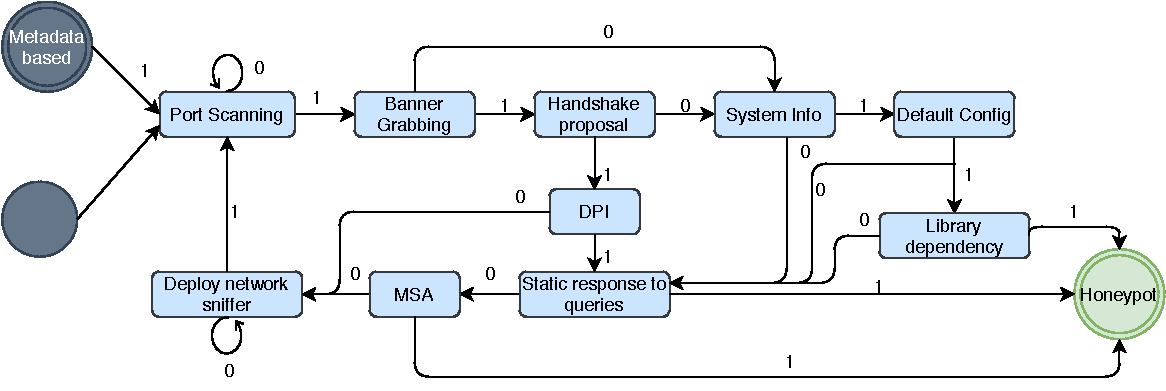
\includegraphics[scale=0.4]{Probe_FSM}
    \caption{\acrshort{fsm} for Probe-Based Fingerprinting}
    \label{fig:probe_fsm}
\end{figure}



\subsubsection{\acrshort{fsm} for Metadata-based Methods}
\label{sec:metadata_fsm}
The \acrshort{fsm} is constructed based on metadata-based fingerprinting methods listed in Figure\ref{fig:taxonomy}. We explain the \acrshort{fsm} created for honeypot fingerprinting in this section. Figure \ref{fig:fsm_md} shows the \acrshort{fsm} created for evaluation of metadata-based methods. The \acrshort{fsm} consists of multiple states with transitions. The states are denoted by the rectangle boxes and the arrows between the boxes denote the transitions. The solid sphere indicates the start state. The green and the red spheres indicate the final states. The numbers zero and one represent true and false. If the metadata based methods were successfully able to extract metadata that can be used for honeypot fingerprinting, we represent the transition as true. If there was no metadata inferred we denote the transition as false. 

We explain the states and the transitions in the \acrshort{fsm} as follows. We begin the process by scanning Shodan and Censys for vulnerable systems exposed to the Internet with SSH, HTTP, MODBUS and Telnet services. The information retrieved from the scan engines is compiled to fingerprint honeypots.With the \acrshort{ip} address of the systems, we can successfully derive the \acrshort{fqdn},Geo-location, hosting provider, \acrshort{isp} of the target system. We use this information in the following states to determine the existence of a honeypot. However, if the metadata is not sufficient to fingerprint, we use this data effectively in the Probe-based methods. 

\begin{figure}[]
    \centering
    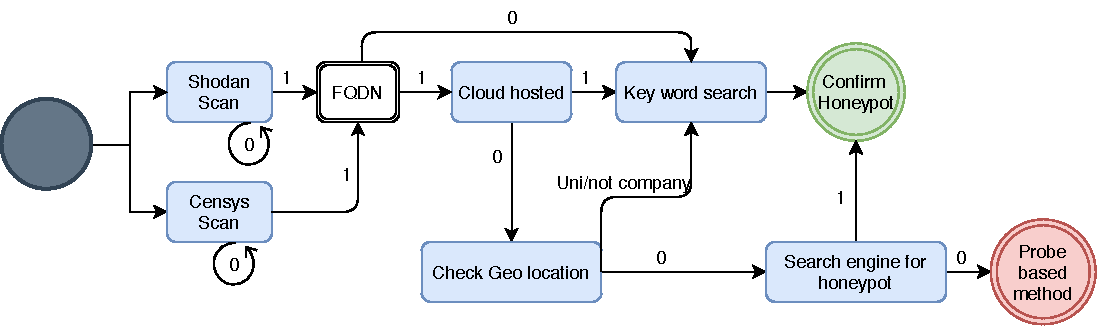
\includegraphics[scale=0.45]{Metadata_FSM}
    \caption{\acrshort{fsm} for Metadata-Based Fingerprinting }
    \label{fig:fsm_md}
\end{figure}


\subsection{Evaluation - Probe-based Techniques}
Probe-based techniques require creation of probes to retrieve specific information from the target system. The probes are constructed based on the techniques Probe-based methods depicted in Figure\ref{fig:taxonomy}. We evaluate the methods by developing a fingerprinting tool based on an \acrfull{fsm} model. The \acrshort{fsm} provides a formal approach to the probing process and the aggregation of data received for honeypot fingerprinting. The \acrshort{fsm} for the probe-based techniques is shown in Figurexxx. 


\subsection{Evaluation - Metadata-based Techniques}
Metadata-based techniques leverage the data that is collected without direct interaction with the honeypot. By implementing crawler described in Section \ref{sec:metadata_fsm} we try to fingerprint honeypots on the Internet. We were successfully able to detect and fingerprint around xxx honeypots. The results are summarized in Table xxx.  


